\documentclass{article}
\usepackage[utf8]{inputenc}
\usepackage{fancyhdr}
\usepackage[margin=2.8cm,twoside]{geometry}
\usepackage[super]{nth}
\usepackage[english]{babel}
\usepackage{csquotes}

\usepackage{hyperref}
\usepackage[backend=biber,style=ieee]{biblatex}
\addbibresource{bibliography.bib}

\usepackage{float}

\pagestyle{fancy}
\fancyhf{}
\fancyhead[LE,RO]{DID - 04 Preliminary Design (Hebb \& Stephan)}
\fancyhead[LO,RE]{\leftmark}
\fancyfoot[LE,RO]{\thepage}

\usepackage{graphicx}

\begin{document}
	
\begin{titlepage}
	\begin{center}
		\vspace*{1cm}
		
		\LARGE\textsc{Royal Military College of Canada}\normalsize
		
		\vspace{0.2cm}
		
		\textsc{Department of Electrical and Computer Engineering}
		
		\vspace{1.5cm}
		
		\includegraphics[width=0.3\textwidth]{rmcLogo.png}
		
		\vspace{1.5cm}
		
		\LARGE{Designing Coatimunde\\}
		
		\vspace{0.2cm}
		
		\normalsize{Computer Optics Analyzing Trajectories In Mostly Unknown, Navigation Denied, Environments}
		
		\vspace{0.1cm}
		
		\normalsize{DID-06 - Schedule Update}
		
		\vfill
		
		\textbf{Presented by:}\\Amos Navarre \textsc{Hebb} \& Kara \textsc{Stephan}\\
		\vspace{0.8cm}
		\textbf{Presented to:}\\Captain Anthony \textsc{Marasco} \& Dr. Rachid \textsc{Beguenane}
		\vspace{0.8cm}
		
		\today
		
	\end{center}
\end{titlepage}



	\section{Document Purpose}
	
	The purpose of this document is to describe the requirements for the Schedule Update. It includes both a graphical and textual representation of the present current project schedule and identifies some schedule risk items.
	
	\section{Changes}
	
	The major cause of delay for our project is the proper identification of the targets and the robot's ability to move towards said target with obstacles. In the updated schedule, \ref{fig:SUp01}, it can be seen that the deadline for this task has been extended. Thus shortening the time we have to port to UAV later in the semester. This task is on the critical path for our project as the next task which is avoiding obstacles and moving towards an identified target with memory of past movements is dependent on the completion of this current task.
	
	\begin{figure}[H]
		\centering
		\includegraphics[width=\linewidth]{SUp01}
		\caption{Textual Representation of Schedule}
		\label{fig:SUp01}
	\end{figure}

	\begin{figure}[H]
		\centering
		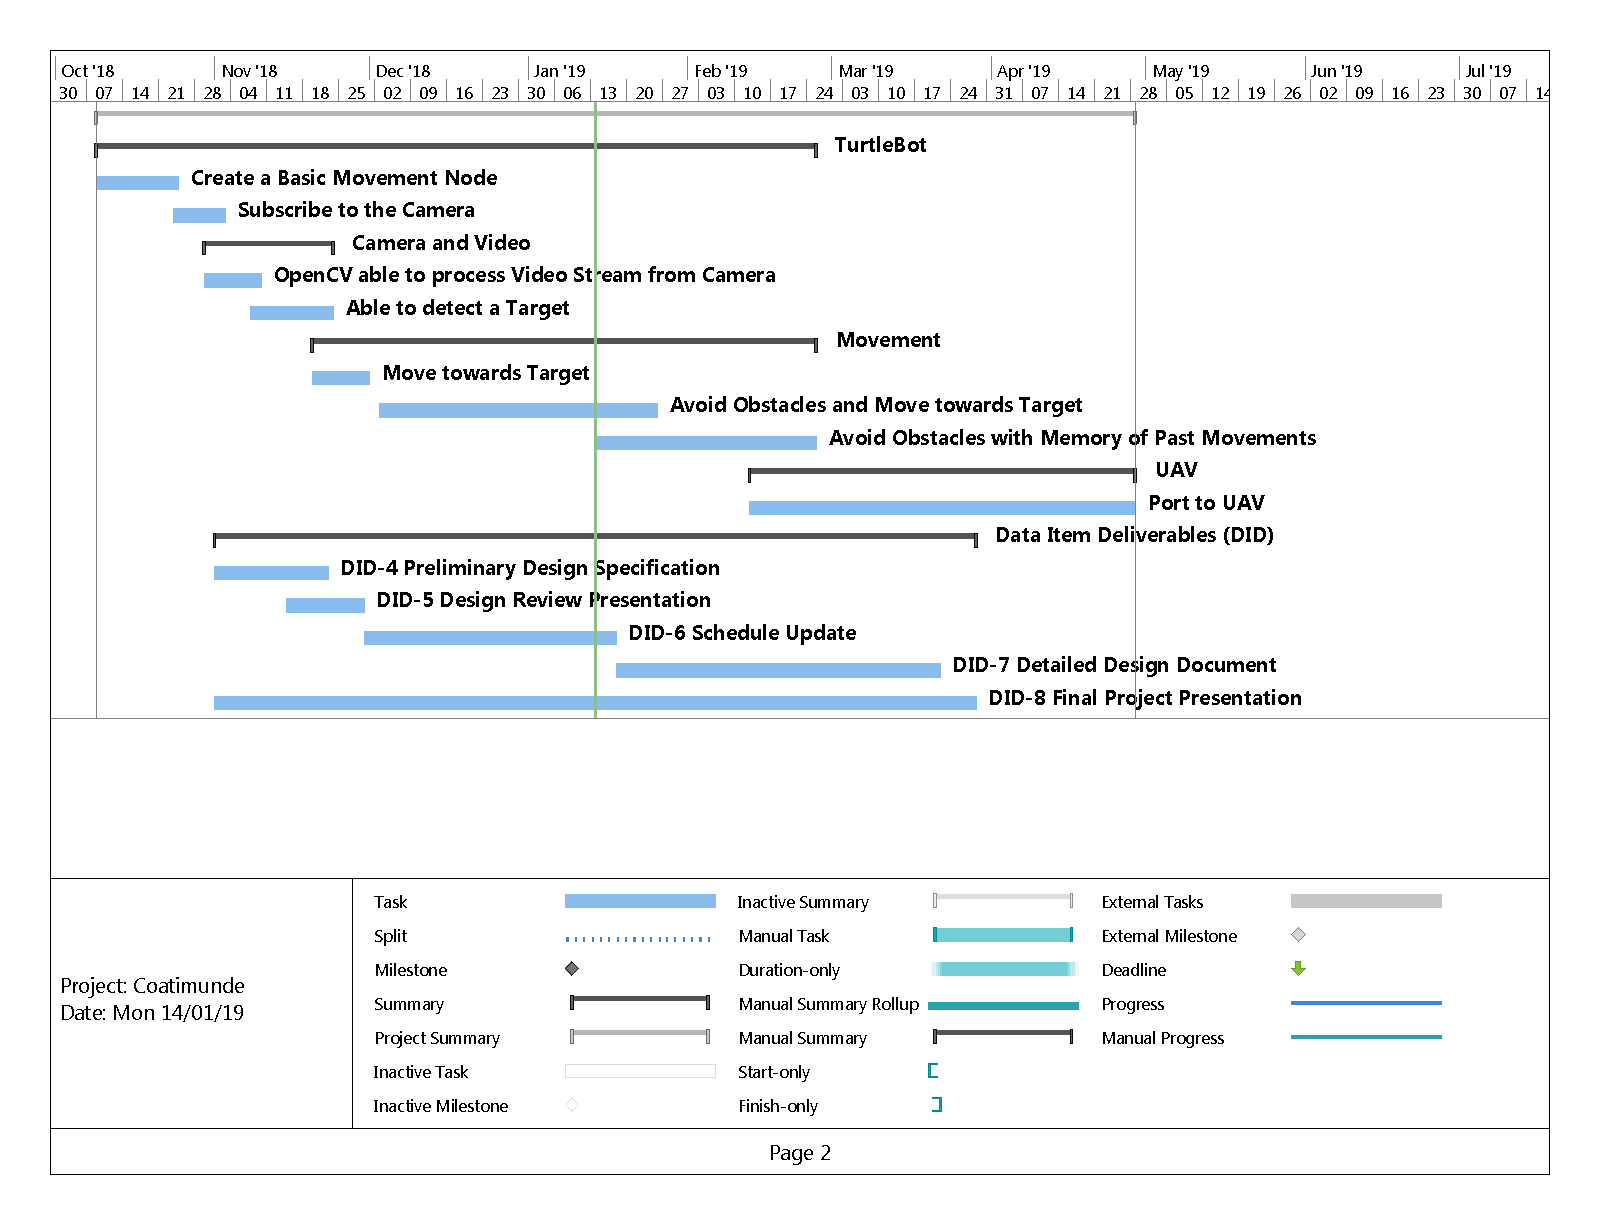
\includegraphics[width=\linewidth]{SUp02}
		\caption{Graphical Representation of Schedule}
		\label{fig:SUp02}
	\end{figure}


\section{Conclusion}

	Underestimating the difficulty of implementing even simple computer vision has resulted in significant delays. We intend to abstract away more of the control and use pre-existing modules in the event that there does not end up being as much time as we desire to port our logic to a flying platform.


%\end{multicols}
\end{document}    

